
%% bare_jrnl_transmag.tex
%% V1.4
%% 2012/12/27
%% by Michael Shell
%% see http://www.michaelshell.org/
%% for current contact information.
%%
%% This is a skeleton file demonstrating the use of IEEEtran.cls
%% (requires IEEEtran.cls version 1.8 or later) with an IEEE 
%% Transactions on Magnetics journal paper.
%%
%% Support sites:
%% http://www.michaelshell.org/tex/ieeetran/
%% http://www.ctan.org/tex-archive/macros/latex/contrib/IEEEtran/
%% and
%% http://www.ieee.org/



% *** Authors should verify (and, if needed, correct) their LaTeX system  ***
% *** with the testflow diagnostic prior to trusting their LaTeX platform ***
% *** with production work. IEEE's font choices can trigger bugs that do  ***
% *** not appear when using other class files.                            ***
% The testflow support page is at:
% http://www.michaelshell.org/tex/testflow/


%%*************************************************************************
%% Legal Notice:
%% This code is offered as-is without any warranty either expressed or
%% implied; without even the implied warranty of MERCHANTABILITY or
%% FITNESS FOR A PARTICULAR PURPOSE! 
%% User assumes all risk.
%% In no event shall IEEE or any contributor to this code be liable for
%% any damages or losses, including, but not limited to, incidental,
%% consequential, or any other damages, resulting from the use or misuse
%% of any information contained here.
%%
%% All comments are the opinions of their respective authors and are not
%% necessarily endorsed by the IEEE.
%%
%% This work is distributed under the LaTeX Project Public License (LPPL)
%% ( http://www.latex-project.org/ ) version 1.3, and may be freely used,
%% distributed and modified. A copy of the LPPL, version 1.3, is included
%% in the base LaTeX documentation of all distributions of LaTeX released
%% 2003/12/01 or later.
%% Retain all contribution notices and credits.
%% ** Modified files should be clearly indicated as such, including  **
%% ** renaming them and changing author support contact information. **
%%
%% File list of work: IEEEtran.cls, IEEEtran_HOWTO.pdf, bare_adv.tex,
%%                    bare_conf.tex, bare_jrnl.tex, bare_jrnl_compsoc.tex,
%%                    bare_jrnl_transmag.tex
%%*************************************************************************

% Note that the a4paper option is mainly intended so that authors in
% countries using A4 can easily print to A4 and see how their papers will
% look in print - the typesetting of the document will not typically be
% affected with changes in paper size (but the bottom and side margins will).
% Use the testflow package mentioned above to verify correct handling of
% both paper sizes by the user's LaTeX system.
%
% Also note that the "draftcls" or "draftclsnofoot", not "draft", option
% should be used if it is desired that the figures are to be displayed in
% draft mode.
%

\documentclass[draftclsnofoot]{IEEEtran}

%\usepackage{cite}
% *** GRAPHICS RELATED PACKAGES ***
%
\ifCLASSINFOpdf
  \usepackage[pdftex]{graphicx}
  % declare the path(s) where your graphic files are
  % \graphicspath{{../pdf/}{../jpeg/}}
  % and their extensions so you won't have to specify these with
  % every instance of \includegraphics
  % \DeclareGraphicsExtensions{.pdf,.jpeg,.png}
\else
  % or other class option (dvipsone, dvipdf, if not using dvips). graphicx
  % will default to the driver specified in the system graphics.cfg if no
  % driver is specified.
  \usepackage[dvips]{graphicx}
  % declare the path(s) where your graphic files are
  % \graphicspath{{../eps/}}
  % and their extensions so you won't have to specify these with
  % every instance of \includegraphics
  % \DeclareGraphicsExtensions{.eps}
\fi
% graphicx was written by David Carlisle and Sebastian Rahtz. It is
% required if you want graphics, photos, etc. graphicx.sty is already
% installed on most LaTeX systems. The latest version and documentation
% can be obtained at: 
% http://www.ctan.org/tex-archive/macros/latex/required/graphics/
% Another good source of documentation is "Using Imported Graphics in
% LaTeX2e" by Keith Reckdahl which can be found at:
% http://www.ctan.org/tex-archive/info/epslatex/
%
% latex, and pdflatex in dvi mode, support graphics in encapsulated
% postscript (.eps) format. pdflatex in pdf mode supports graphics
% in .pdf, .jpeg, .png and .mps (metapost) formats. Users should ensure
% that all non-photo figures use a vector format (.eps, .pdf, .mps) and
% not a bitmapped formats (.jpeg, .png). IEEE frowns on bitmapped formats
% which can result in "jaggedy"/blurry rendering of lines and letters as
% well as large increases in file sizes.
%
% You can find documentation about the pdfTeX application at:
% http://www.tug.org/applications/pdftex


% *** MATH PACKAGES ***
%
\usepackage[cmex10]{amsmath}
% A popular package from the American Mathematical Society that provides
% many useful and powerful commands for dealing with mathematics. If using
% it, be sure to load this package with the cmex10 option to ensure that
% only type 1 fonts will utilized at all point sizes. Without this option,
% it is possible that some math symbols, particularly those within
% footnotes, will be rendered in bitmap form which will result in a
% document that can not be IEEE Xplore compliant!
%
% Also, note that the amsmath package sets \interdisplaylinepenalty to 10000
% thus preventing page breaks from occurring within multiline equations. Use:
%\interdisplaylinepenalty=2500
% after loading amsmath to restore such page breaks as IEEEtran.cls normally
% does. amsmath.sty is already installed on most LaTeX systems. The latest
% version and documentation can be obtained at:
% http://www.ctan.org/tex-archive/macros/latex/required/amslatex/math/





% *** SPECIALIZED LIST PACKAGES ***
%
%\usepackage{algorithmic}
% algorithmic.sty was written by Peter Williams and Rogerio Brito.
% This package provides an algorithmic environment fo describing algorithms.
% You can use the algorithmic environment in-text or within a figure
% environment to provide for a floating algorithm. Do NOT use the algorithm
% floating environment provided by algorithm.sty (by the same authors) or
% algorithm2e.sty (by Christophe Fiorio) as IEEE does not use dedicated
% algorithm float types and packages that provide these will not provide
% correct IEEE style captions. The latest version and documentation of
% algorithmic.sty can be obtained at:
% http://www.ctan.org/tex-archive/macros/latex/contrib/algorithms/
% There is also a support site at:
% http://algorithms.berlios.de/index.html
% Also of interest may be the (relatively newer and more customizable)
% algorithmicx.sty package by Szasz Janos:
% http://www.ctan.org/tex-archive/macros/latex/contrib/algorithmicx/




% *** ALIGNMENT PACKAGES ***
%
%\usepackage{array}
% Frank Mittelbach's and David Carlisle's array.sty patches and improves
% the standard LaTeX2e array and tabular environments to provide better
% appearance and additional user controls. As the default LaTeX2e table
% generation code is lacking to the point of almost being broken with
% respect to the quality of the end results, all users are strongly
% advised to use an enhanced (at the very least that provided by array.sty)
% set of table tools. array.sty is already installed on most systems. The
% latest version and documentation can be obtained at:
% http://www.ctan.org/tex-archive/macros/latex/required/tools/


% IEEEtran contains the IEEEeqnarray family of commands that can be used to
% generate multiline equations as well as matrices, tables, etc., of high
% quality.




% *** SUBFIGURE PACKAGES ***
%\ifCLASSOPTIONcompsoc
%  \usepackage[caption=false,font=normalsize,labelfont=sf,textfont=sf]{subfig}
%\else
%  \usepackage[caption=false,font=footnotesize]{subfig}
%\fi
% subfig.sty, written by Steven Douglas Cochran, is the modern replacement
% for subfigure.sty, the latter of which is no longer maintained and is
% incompatible with some LaTeX packages including fixltx2e. However,
% subfig.sty requires and automatically loads Axel Sommerfeldt's caption.sty
% which will override IEEEtran.cls' handling of captions and this will result
% in non-IEEE style figure/table captions. To prevent this problem, be sure
% and invoke subfig.sty's "caption=false" package option (available since
% subfig.sty version 1.3, 2005/06/28) as this is will preserve IEEEtran.cls
% handling of captions.
% Note that the Computer Society format requires a larger sans serif font
% than the serif footnote size font used in traditional IEEE formatting
% and thus the need to invoke different subfig.sty package options depending
% on whether compsoc mode has been enabled.
%
% The latest version and documentation of subfig.sty can be obtained at:
% http://www.ctan.org/tex-archive/macros/latex/contrib/subfig/



% *** FLOAT PACKAGES ***
%
% \usepackage{fixltx2e}
% fixltx2e, the successor to the earlier fix2col.sty, was written by
% Frank Mittelbach and David Carlisle. This package corrects a few problems
% in the LaTeX2e kernel, the most notable of which is that in current
% LaTeX2e releases, the ordering of single and double column floats is not
% guaranteed to be preserved. Thus, an unpatched LaTeX2e can allow a
% single column figure to be placed prior to an earlier double column
% figure. The latest version and documentation can be found at:
% http://www.ctan.org/tex-archive/macros/latex/base/


\usepackage{stfloats}
% stfloats.sty was written by Sigitas Tolusis. This package gives LaTeX2e
% the ability to do double column floats at the bottom of the page as well
% as the top. (e.g., "\begin{figure*}[!b]" is not normally possible in
% LaTeX2e). It also provides a command:
%\fnbelowfloat
% to enable the placement of footnotes below bottom floats (the standard
% LaTeX2e kernel puts them above bottom floats). This is an invasive package
% which rewrites many portions of the LaTeX2e float routines. It may not work
% with other packages that modify the LaTeX2e float routines. The latest
% version and documentation can be obtained at:
% http://www.ctan.org/tex-archive/macros/latex/contrib/sttools/
% Do not use the stfloats baselinefloat ability as IEEE does not allow
% \baselineskip to stretch. Authors submitting work to the IEEE should note
% that IEEE rarely uses double column equations and that authors should try
% to avoid such use. Do not be tempted to use the cuted.sty or midfloat.sty
% packages (also by Sigitas Tolusis) as IEEE does not format its papers in
% such ways.
% Do not attempt to use stfloats with fixltx2e as they are incompatible.
% Instead, use Morten Hogholm'a dblfloatfix which combines the features
% of both fixltx2e and stfloats:
%
% \usepackage{dblfloatfix}
% The latest version can be found at:
% http://www.ctan.org/tex-archive/macros/latex/contrib/dblfloatfix/



\ifCLASSOPTIONcaptionsoff
  \usepackage[nomarkers]{endfloat}
 \let\MYoriglatexcaption\caption
 \renewcommand{\caption}[2][\relax]{\MYoriglatexcaption[#2]{#2}}
\fi
% endfloat.sty was written by James Darrell McCauley, Jeff Goldberg and 
% Axel Sommerfeldt. This package may be useful when used in conjunction with 
% IEEEtran.cls'  captionsoff option. Some IEEE journals/societies require that
% submissions have lists of figures/tables at the end of the paper and that
% figures/tables without any captions are placed on a page by themselves at
% the end of the document. If needed, the draftcls IEEEtran class option or
% \CLASSINPUTbaselinestretch interface can be used to increase the line
% spacing as well. Be sure and use the nomarkers option of endfloat to
% prevent endfloat from "marking" where the figures would have been placed
% in the text. The two hack lines of code above are a slight modification of
% that suggested by in the endfloat docs (section 8.4.1) to ensure that
% the full captions always appear in the list of figures/tables - even if
% the user used the short optional argument of \caption[]{}.
% IEEE papers do not typically make use of \caption[]'s optional argument,
% so this should not be an issue. A similar trick can be used to disable
% captions of packages such as subfig.sty that lack options to turn off
% the subcaptions:
% For subfig.sty:
% \let\MYorigsubfloat\subfloat
% \renewcommand{\subfloat}[2][\relax]{\MYorigsubfloat[]{#2}}
% However, the above trick will not work if both optional arguments of
% the \subfloat command are used. Furthermore, there needs to be a
% description of each subfigure *somewhere* and endfloat does not add
% subfigure captions to its list of figures. Thus, the best approach is to
% avoid the use of subfigure captions (many IEEE journals avoid them anyway)
% and instead reference/explain all the subfigures within the main caption.
% The latest version of endfloat.sty and its documentation can obtained at:
% http://www.ctan.org/tex-archive/macros/latex/contrib/endfloat/
%
% The IEEEtran \ifCLASSOPTIONcaptionsoff conditional can also be used
% later in the document, say, to conditionally put the References on a 
% page by themselves.


% *** PDF, URL AND HYPERLINK PACKAGES ***
%
\usepackage{url}
% url.sty was written by Donald Arseneau. It provides better support for
% handling and breaking URLs. url.sty is already installed on most LaTeX
% systems. The latest version and documentation can be obtained at:
% http://www.ctan.org/tex-archive/macros/latex/contrib/url/
% Basically, \url{my_url_here}.




% *** Do not adjust lengths that control margins, column widths, etc. ***
% *** Do not use packages that alter fonts (such as pslatex).         ***
% There should be no need to do such things with IEEEtran.cls V1.6 and later.
% (Unless specifically asked to do so by the journal or conference you plan
% to submit to, of course. )


% correct bad hyphenation here
\hyphenation{op-tical net-works semi-conduc-tor}

\usepackage{caption} % http://ctan.org/pkg/caption
\usepackage{booktabs}
\usepackage{enumitem}

\begin{document}

\markboth{Chimakurthi et al.}{Business Dynamics and Neighborhood Characteristics: Update 1}

\title{Understand Local Business Dynamics and Neighborhood Characteristics with Yelp Data: \textsc{Update \#1}} % title

\author{Lakshmimanaswitha Chimakurthi, Zexi Han, Anant Jain, Jianchao Yang}

% As a general rule, do not put math, special symbols or citations
% in the abstract or keywords.
\IEEEtitleabstractindextext{%
\begin{abstract}
The goal of our project is to use Yelp data to describe business dynamics, and use neighborhood characteristics to explain such  dynamics. During the first phrase of our work, we have explored our dataset in detail, defined the subset of the data we want to work with, identified interesting features, from both the Yelp and public datasets, and constructed an example feature matrix, which we then demonstrate how we are going to use it for clustering.
\end{abstract}

% Note that keywords are not normally used for peerreview papers.
\begin{IEEEkeywords}
local businesses, urban dynamics, exploratory data analysis
\end{IEEEkeywords}}


% make the title area
\maketitle


% To allow for easy dual compilation without having to reenter the
% abstract/keywords data, the \IEEEtitleabstractindextext text will
% not be used in maketitle, but will appear (i.e., to be "transported")
% here as \IEEEdisplaynontitleabstractindextext when the compsoc 
% or transmag modes are not selected <OR> if conference mode is selected 
% - because all conference papers position the abstract like regular
% papers do.
\IEEEdisplaynontitleabstractindextext
% \IEEEdisplaynontitleabstractindextext has no effect when using
% compsoc or transmag under a non-conference mode.


\section{Explore the Yelp Data}

\IEEEPARstart{A}{s} reported earlier:

\begin{quote}
The [Yelp Dataset] comprise of more than 156,000 businesses distributed over 12 metropolitan areas; over 4,700,000 reviews, 200,000 pictures, 1,000,000 tips by 1,100,000 users; and aggregated hourly check-in counts for each day of a week. The metadata comprises of over 1.2 million business attributes like hours, parking, availability, and ambience. In addition, some additional metadata fields like user ratings, categories, user captions and geo-coordinates are listed.
\end{quote}

With such vast amount and variety of data, we must limit our work to a subset of the data, and pick only the features of our interests.

\subsection{Pick the right cities}

The Yelp dataset has businesses from 1,010 different cities (including duplicate city names due to spelling inconsistencies). It would be impracticable to collect neighborhood characteristics data for all of these citiess. Since $73.48\%$ of the businesses are located in the US, we will focus on cities in the US only.

\begin{figure}[h]
  \hspace{-.5em}
    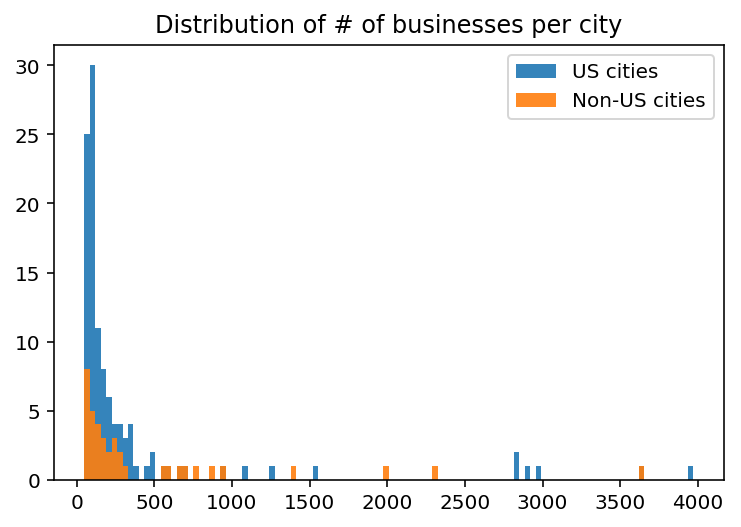
\includegraphics[width=0.5\textwidth]{hist-city-biz}
  \caption{Number of businesses for US and Non-US cities}
  \label{city-biz}
\end{figure}

As displayed in Fig. \ref{city-biz}, in this dataset, most cities have less than 500 businesses (the graph already excluded cities with less than 50 businesses). The Top 10 cities with most businesses are shown in Table \ref{city-biz-table}.

\begin{table}[htbp]
\caption{Top cities with most businesses}
\label{city-biz-table}
\centering
\begin{tabular}{llrrrr}
\toprule
{} &        city &      n &  \% open &  n\_review\_avg &  stars\_avg \\
\midrule
0 &   Las Vegas &  24768 &    0.83 &         58.80 &       3.71 \\
1 &     Phoenix &  15656 &    0.85 &         33.17 &       3.68 \\
2 &   Charlotte &   7557 &    0.85 &         28.07 &       3.58 \\
3 &  Scottsdale &   7510 &    0.82 &         37.24 &       3.94 \\
4 &  Pittsburgh &   5688 &    0.84 &         28.54 &       3.66 \\
5 &        Mesa &   5146 &    0.88 &         22.43 &       3.63 \\
6 &   Henderson &   4130 &    0.85 &         35.73 &       3.78 \\
7 &       Tempe &   3949 &    0.81 &         37.49 &       3.71 \\
8 &    Chandler &   3649 &    0.84 &         29.93 &       3.75 \\
9 &   Cleveland &   2979 &    0.84 &         28.38 &       3.61 \\
\bottomrule
\end{tabular}
\end{table}

One thing to note is that this dataset does not contain all businesses for any given city. For example, Las Vegas has 79,173 businesses when searching directly on the Yelp website, but this dataset contains only 24,768. That is less than one third of all available businesses. We shall keep this in mind when trying to interpret the results for neighborhoods with smaller populations.

We have decided to work on only the Top 30 US cities in terms of number of businesses. The 30st city is Monroeville, PA, which is within Pittsburgh metropolitan area and has a population of 28,000 people. The Yelp dataset has 316 businesses in it. 316 is a decent number for a small city like this.

\subsection{Pick the right features}

This dataset contains some closed businesses (as indicated by the \textit{\% open} column in Table \ref{city-biz-table}). Overall, there are about 15\% businesses have closed their doors forever. The dataset still contains user activities for them, such as reviews and tips users left. An idea for future analysis is to compute the average life-span of a closed business (the time from when it received its first user activity, be it a review or a tip, till it received the last one.), then use it as an indicator for the viability of businesses in a neighborhood.

For now, we focus on features that are relatively easy to extract.

All of our features are aggregated by neighborhood. The \texttt{businesses} table in Yelp data has a \texttt{neighborhood} column, but it is missing values for many businesses (nearly two thirds of all records).

Despite this incompleteness of the data, we still tried to aggregate features with this column, just to get the feature building process started. Nevertheless, the missing observations were not particularly biased anyway. If we plot businesses with neighborhoods information for the largest city we have--Las Vegas, we can clearly see a more or less identical distribution of the businesses, comparing to what we get from plotting all businesses.

\begin{figure}[h]
  \centering
    \includegraphics[trim=45 0 0 0,clip,width=0.5\textwidth]{vegas-neighborhoods-1}
  \caption{Businesses of Las Vegas by Neighborhoods}
  \label{vegas-neighborhoods}
\end{figure}

In the future, we will map each business to a Census Track, Census Block Group, or ZIP code, using the coordinates of the businesses and the geographic boundaries of these neighborhood units. This is necessary because neighborhood characteristics, such as demographics and economy indicators, are all reported to the census tract or ZIP code level.

The features we have extracted include:

\begin{itemize}
	\item Average review count of all businesses in a neighborhood.
	\item Average star ratings of the businesses.
	\item Number of unique service categories represented by all businesses in a neighborhood (diversity of businesses).
	\item Number of businesses in each of the Top 10 to 20 categories. Each category as a feature.
\end{itemize}

Some basic statistics of the first three features are shown in Table \ref{feature-stats}.

\begin{table}[htbp]
\caption{Statistics of basic features}
\label{feature-stats}
\centering
\begin{tabular}{lrrr}
\toprule
{} &  n\_review\_avg &  stars\_avg   &  n\_uniq\_categories \\
\midrule
mean  &             25.43 &       3.69 &          108.92 \\
std   &             39.85 &       0.48 &          140.81 \\
min   &              3.00 &       1.50 &            2.00 \\
25\%   &              9.87 &       3.50 &           21.00 \\
50\%   &             17.55 &       3.71 &           55.00 \\
75\%   &             31.74 &       3.91 &          135.00 \\
max   &            544.00 &       5.00 &          771.00 \\
\bottomrule
\end{tabular}
\end{table}

There are in total 1,101 categories in this dataset. Categories are hierarchical and often overlaps with each other. So we treat them as tags. The Top 10 categories are displayed in Table \ref{top-cats}.

\begin{table}[htbp]
\caption{Top business categories}
\label{top-cats}
\centering
\begin{tabular}{lr}
\toprule
Category &  	Count \\
\midrule
Restaurants      &           10096 \\
Shopping         &            5725 \\
Food             &            4871 \\
Beauty \& Spas    &            3725 \\
Nightlife        &            3097 \\
Health \& Medical &            2996 \\
Home Services    &            2954 \\
Bars             &            2541 \\
Local Services   &            2174 \\
Automotive       &            2002 \\
\bottomrule
\end{tabular}
\end{table}

Among 35,048 businesses we filtered out (those located in the US and containing neighborhood information), 10,096 of them are restaurants. Despite Yelp mainly known for its restaurant reviews, we still get a decent number of other types of services.

\section{Collect neighborhood characteristics data}

\url{Census.org} is our main resource for neighborhood characteristics data. After filtering the dataset by cities, we obtain the list of relevant states (AZ NV NC PA OH WI IL SC), then download the cartographic boundary shapefiles for each state from the US Census Bureau website \footnote{\url{https://www.census.gov/geo/maps-data/data/tiger-cart-boundary.html}}.

We then use the \texttt{census} package to collect census data for all  top 30 cities we have filtered out.

The list of available census variables can be found at \url{censusreporter.org}.

The variables we have collected include proportion of residents by race, age group, education attainment, nationality, marital status, housing condition (renters v.s. home owners), commuting time to work, whether live below poverty line or not, whether received any sort of public assistance or not, and median house income.

Census data are be good enough for our initial exploration of neighborhood characteristics. We may incorporate more data sources as it seems fit.

\section{Explore more of the Yelp Data}

We have surveyed the potential of other Yelp data tables, too.

\subsection{User reviews and tips}

Using wordcloud graphs (Fig. \ref{reviews-wordcloud}), we are able to see the common keywords in users reviews and tips.

\begin{figure}[h]
\hspace{-.5em}
\includegraphics[width=0.5\textwidth]{reviews-wordcloud}
\caption{Word cloud for reviews}
\label{reviews-wordcloud}
\end{figure}

\begin{figure}[h]
\hspace{-.5em}
\includegraphics[width=0.5\textwidth]{tips-wordcloud}
\caption{Word cloud for tips}
\label{tips-wordcloud}
\end{figure}

Positive comments such as "good place", "great food" are common in both reviews and tips. It seems that there really isn't much distinction in terms of the content between reviews and tips. It could be users are writing tips like "short reviews", expressing their positive experience, rather than providing actual helpful tips to fellow customers; or users always add some comments regarding their experience while providing tips.

We expect the sentiment metric derived from reviews to be very much in line with the star ratings, so text analysis based on reviews would be low priority for now.

\subsection{Checkins}

The \texttt{checkin} table does not contain detailed checkin records of all users, but rather the count of checkins at each hour of the day of the week for each businesse.

This theoretically can be used to represent the popularity of the businesses. We can then construct a feature indicating whether a neighborhood has more vibrant business activities than the city average during weekends. But this feature might not bear too much power due to the lack of checkins for too many businesses.

\subsection{Users}

The \texttt{user} table has 22 features about a user's first name, review count, registration date, list of friends, and some aggregation metrics about how many votes and compliments they sent to and received from other Yelp users.

We do not know where do users live, but we are able to identify those who made a review to a business located in the US. In total, US businesses have received 1,768,297 reviews from 560,547 users.

Among all the users, 4.7\% were selected as elite users for at least one year.

Future work may include identify patronage of elite users for businesses. E.g., percentage of reviews written by elite users.

\section{Test clustering}

Using the three basic features, together with number of businesses in 10 top categories, we build a $225\times13$ feature matrix, then use k-means to identify the clusters.

The elbow method indicates the optimal cluster number is 3 for this sample feature set (Fig. \ref{elbow}).

Fig. \ref{corr} shows the correlation of these features. Unsurprisingly, most of them are highly correlated, except for many bars and nightlife. Future work will employ dimension reduction for these categories, as many of them are even just aliases to each other.
 
\begin{figure}[htbp]
\centering
\includegraphics[width=0.4\textwidth]{elbow}
\caption{Number of clusters and distortions}
\label{elbow}
\end{figure}

\begin{figure}[htbp]
\centering
\includegraphics[width=0.4\textwidth]{corr}
\caption{Correlation of 13 features}
\label{corr}
\end{figure}

\begin{table*}[htbp]
\caption{Centroids after Clustering}
\label{cluster-centroids}
\begin{tabular}{lrrrrrrrrrrrrr}
\toprule
{} &  auto &  bars &  beauty &  food &  health &  home &  local &  night &  restaur & reviews &  shopping &  uniq\_cat &  stars \\
\midrule
cluster 0 &        142.33 &  167.00 &        279.83 &  304.17 &           242.33 &          212.67 &           158.67 &       224.67 &         624.17 &         68.77 &      474.33 &               641.00 &       3.70 \\
cluster 1 &          2.05 &    2.30 &          1.66 &    4.28 &             1.09 &            1.84 &             1.58 &         2.68 &           9.49 &         20.69 &        3.15 &                50.07 &       3.68 \\
cluster 2 &         19.53 &   28.18 &         43.72 &   57.00 &            33.65 &           33.73 &            23.50 &        31.73 &         116.33 &         40.11 &       57.90 &               292.45 &       3.72 \\
\bottomrule
\end{tabular}
\end{table*}

Looking at the identified centroids (Table \ref{cluster-centroids}), the most determining factors are unavoidably the number of businesses. Even number of reviews per business is positively correlated with number of businesses in a neighborhood, too. We have effectively clustered the neighborhoods based on their sizes.

We shall be able to capture a different pattern had those big neighborhoods were split into smaller geographic units.

\section{Future work}

As discussed in previous sections, we still have much work to do. Here is a (semi-)complete list:

\begin{enumerate}[label=\arabic*.]
	\item Map businesses to census tracts.
	\item Aggregate measures at the census tract level.
	\item Extract features from business attributes (price range, amenities, open hours, etc).
	\item Extract features from reviews and checkins (proportion of reviews made by elite users, popular on weekends, etc).
	\item Reduce dimension of the features.
	\item Add neighborhood characteristics to clustering.
	\item Explain the clusters.
\end{enumerate}


\end{document}
